\chapter{Implementation}
\label{chap:implementation}

% In diesem Kapitel beschreiben Sie Ihre Lösung des Problems. Geben Sie dem Leser genügend Einblick in die Lösung, so dass er Ihre Arbeit entsprechend würdigen kann. Verwenden Sie aber Anhänge für Dinge, die hier nicht unbedingt bis ins letzte Detail verstanden werden müssen.

\section{Komponenten}
\label{sec:komponenten}

\subsection{Stanford Protégé}
\label{subsec:protege}

\subsection{Clark &\ Parsia Stardog}
\label{subsec:stardog}

\subsubsection{Reasoner}
\label{ssubsec:reasoner}
Reasoner sind Komponenten, welche eine Folgerung von implizitem Wissen zulassen bzw.\ bieten. Es handelt es sich um eine Art ``Verstehen'' durch Maschinen. Man möchte also implizite Fakten finden, welche durch explizite Fakten in einer Ontologie definiert sind. 

Als Reasoner kommt Pellet zum Einsatz. Dabei handelt es sich um einen Reasoner, für die Sprache OWL-DL~\footnote{http://www.w3.org/TR/owl-ref/\#OWLDL}, welche wiederum eine Teilsprache von OWL darstellt. Eine komplette Unterstützung des OWL full Profils ist so nicht möglich, da dieses nicht entscheidbar ist, daher beschränkt sich die Umsetzung auf OWL DL\@. Pellet setzt dabei komplett die Spezifikation der WebOnt Arbeitsgruppe um. OWL-DL ist eine syntaktische Variante der Beschreibungslogik SHOIN (D).

\begin{figure}[htbp]
\centering \rotatebox{0}{\scalebox{0.5}[0.5]{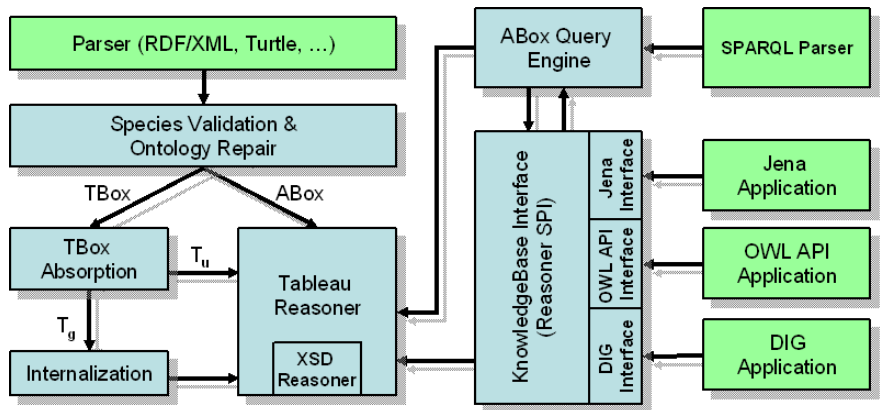
\includegraphics{bilder/pellet_komponenten.png}}}
\caption{Hauptkomponenten des Pellet-Reasoners.\label{fig:pellet_komponenten}\protect\footnotemark}
\end{figure}
\footnotetext{\cite[S. 6]{sirin:pellet05}}

\subsubsection{Beschreibungslogik}
\label{subsubsection:beschreibungslogik}
Beschreibungslogiken sind Formalismen um Wissen darzustellen, dabei sind sie eine Teilmenge der Prädikatenlogik. Sie stellen den Kern von Wissensrepräsentationssystemen dar, in dem sie eine Struktur für eine Wissensbasis und den damit verbundenen Methoden zur Folgerung bieten (vgl.~\cite{dl:baader2003}).

Die Struktur, welche Beschreibungslogiken als Wissensbasis bereitstellen, besteht aus einem Schema (Tbox, Regeln), sowie aus den Daten (Abox, Fakten).

Die Semantik von Beschreibungslogiken wird durch Interpretationen definiert:

\noindent\hspace*{16mm} $ I = (\Delta^I, \cdot^I) $

Dabei ist:
\begin{itemize}
\item $ \Delta^I $

    Die (Wissens-) Domäne (eine nicht leere Menge).

\item $ \cdot^I $

    Eine Funktion zur Interpretation von:
    \begin{itemize}
        \item Konzepten (Klassen, A)

            Wobei $ A^I $ eine Teilmenge von $ \Delta^I $ ist.
        \item Rollen (Eigenschaften, R)

            Wobei $ R^I $ eine binäre Relation auf $ \Delta^I $ ist.
        \item Individuen (i)

            Wobei $ i^I $ Element von $ \Delta^I $ ist.
    \end{itemize}
\end{itemize}

Die Funktion zur (Wissens-) Interpretation $ \cdot^I $ definiert, wie atomare Konzpte, Eigenschaften und Individuen zu interpretieren sind. Eine Interpretation, welche allen Axiomen einer Ontologie in Beschreibungslogik genügt ist ein Modell der Ontologie.

Eine Ontologie in Beschreibungslogik ist eine Menge von Termen und deren Relationen. Die Interpretation dieser Ontologie stellt als ein Modell dar, welches die Ontologie abbildet.

Die Pellet zu Grunde liegende Beschreibungslogik SHOIN (D) ist ein Kürzel und steht für:
\begin{itemize}
\item \textit{S}

ALC (Attributive Concept Language with Complements) mit einer transitiven Rolle. Bei ALC handelt es sich um die kleinste Beschreibungslogik, welche aussagenlogisch geschlossen ist (d.h.\ sie bietet, entweder implizit oder explizit, Konjunktion, Union und Negation von Klassen (-beschreibungen)). Eine Rolle entspricht einer Eigenschaft bzw.\ einem Prädikat in der Prädikatenlogik erster Stufe.

\item \textit{H}

    Rollenhierarchie (Sub-Eigenschaften), z.B. rdfs:subPropertyOf.

\item \textit{O}

    Nominal, z.B. Wochenden = {Samstag, Sonntag}.


\item \textit{I}

    Inverse Rolle (inverse Eigenschaft bzw.\ Prädikt).

\item \textit{N}

    Nummerische Einschränkung, z.B. >= hatKind 1.

\item \textit{(D)}

    Nutzung von Wertebereichen, Werten oder Datentypen.
\end{itemize}

(vgl.~\cite{dl:baader2003})

\subsubsection{Folgerung}
\label{subsubsection:folgerung}
Die W3C Spezifikation betreffend der Umsetzung eines Reasoners definiert zwei Arten von OWL Dokumentprüfungen: Prüfung auf korrekte Syntax sowie Prüfung der Konsistenz. Bei der Konsistenzprüfung geht es darum festzustellen, ob eine gegebene Eingabe anhand einer definierten Spezifikation syntaktisch korrekt ist. Jedoch macht eine reine Umsetzung der genannten Prüfungen wenig Sinn. Man möchte ja eine Ontologie möglichst effektiv nutzen können, zum Beispiel um indirektes Wissen abzuleiten.  Da OWL DL eine syntaktische Variante der Beschreibungslogik SHOIN (D) darstellt, liegt es nahe, mittels einem Reasoner folgende Methoden zur Inferenz zur Verfügung zu stellen:
\begin{itemize}
\item \textit{Konsistenzprüfung}

Stellt sicher, dass sich in der Ontologie keine gegenstätzlichen Fakten befinden. Konkret bedeutet dies anhand der OWL Semantik~\footnote{http://www.w3.org/TR/owl-semantics/}, dass die Konsistenz einer ABox in Bezug auf eine TBox geprüft wird.
\item \textit{Konzept-Erfüllbarkeit}

Stellt sicher, dass Objekte einer Klasse instanziert werden können. Ist dies nicht der Fall, so ist die Ontologie inkonsistent.
\item \textit{Klassifikation}

Berechnet die Relationen zwischen Subklassen, stellt also die Klassenhierarchie auf. Dies ermöglicht das Abfragen der Ontologie.
\item \textit{Gewinnung von Erkenntnissen}

Findet die spezifischste Klasse eines Objektes, leitet also den direkten Typ jedes Objektes ab.
\end{itemize}
(vgl. \citet[S. 1 und 2]{sirin:pellet05})

Bei der eigentliche Komponente, welche in Pellet zur Folgerung eingesetzt wird, handelt es sich um den Tableau Reasoner, welcher den gleichnamigen Algorithmus verwendet. Dieser reduziert ein Problem der Folgerung auf ein Problem der Konzept-Erfüllbarkeit, wobei er eine Interpretation sucht, welche die gefragten Konzepte erfüllt. Solch eine Interpretation wird inkrementell als eine Art Tafel (eben, Tableau) aufgebaut.

Nachfolgend ein Beispiel, gegeben sei:
$ Prolog \subseteq LogischeProgrammiersprache, LogischeProgrammiersprache \subseteq Programmiersprache $
Man stellt nun folgende Anfrage:
$ if Prolog \subseteq Programmiersprache $

Der Prozess der Folgerung findet nun wie folgt statt:
\begin{itemize}
    \item Testen, ob ein Individuum existiert, welches eine logische Programmiersprache, aber keine Programmiersprache ist. Man möchte also die Erfüllbarkeit des Konzeptes $ C_0 = (Prolog \sqcap \neg Programmiersprache) $ testen.
    \item $ C_0(x) \Rightarrow Prolog(x), (\neg Programmiersprache)(x) $
    \item $ Prolog(x) \Rightarrow LogischeProgrammiersprache(x) $
    \item $ LogischeProgrammiersprache(x) \Rightarrow Programmiersprache(x) $
        $ \Rightarrow $ Konflikt!
\end{itemize}
Wie ersichtlich ist, ist das Konzept $ C_0 $ nicht erfüllbar, die Anfrage $ Prolog \subseteq Programmiersprache $ trifft also innerhalb der gegebenen Ontologie zu. Der Beweis wird mittels Kontradiktion erbracht.

Der generelle Prozess der Folgerung läuft wie folgt ab:
\begin{itemize}
    \item Umwandlung eines Konzeptes bzw.\ der Konzepte in die negierte Normalform (NNF), die Negation $ \neg $ befindet sich vor Konzeptnamen.
    \item Ablegen des umgewandelten Konzeptes als $ C_0 $.

        Der Algorithmus hat also die Datenbasis (Abox) $ A_0 = {C_0(x_0)} $
    \item Regeln zur Transformation auf die Datenbasis (Abox) so weit als möglich anwenden.
    \item Wurde eine gültige Datenbasis (Abox) gefunden, so ist $ C_0 $ erfüllbar.
    \item Wurde keine gültige Datenbasis unter Berücksichtigung aller (Such-) Pfade gefunden, so ist $ C_0 $ nicht erfüllbar.
\end{itemize} (vgl.~\cite{horrocks2002} und~\cite{horrocks2005})
